%% ----------------------------------------------------------------
%% Thesis.tex -- MAIN FILE (the one that you compile with LaTeX)
%% ---------------------------------------------------------------- 

%% Manual stuff todo at the end:
% - put the URL addresses in the extra field of the bibtex file in \url{}
% - delete the howpublished items from bibtex file
% - identicon upper/lower case

% Set up the document
\documentclass[a4paper, 11pt, oneside]{thesis}  % Use the "Thesis" style, based on the ECS Thesis style by Steve Gunn
\graphicspath{{figures/}}  % Location of the graphics files (set up for graphics to be in PDF format)

% Microtype
\usepackage[activate={true,nocompatibility},final,kerning=true,spacing=true,factor=1100,stretch=10,shrink=10]{microtype}
% activate={true,nocompatibility} - activate protrusion and expansion
% final - enable microtype; use "draft" to disable
% tracking=true, kerning=true, spacing=true - activate these techniques
% factor=1100 - add 10% to the protrusion amount (default is 1000)
% stretch=10, shrink=10 - reduce stretchability/shrinkability (default is 20/20)

% Include any extra LaTeX packages required
\usepackage{makeidx}
\usepackage[utf8]{inputenc}
\usepackage[english]{babel}
\usepackage{natbib}  % , sort&compress, sort&compress,authoryear, square, comma] Use the "Natbib" style for the references in the Bibliography
\usepackage{verbatim}  % Needed for the "comment" environment to make LaTeX comments
\usepackage{vector}  % Allows "\bvec{}" and "\buvec{}" for "blackboard" style bold vectors in maths
\usepackage[usenames,dvipsnames]{color}
\usepackage{setspace}
\definecolor{DarkGray}{RGB}{90,90,90}
\definecolor{DarkDarkBlue}{RGB}{0,40,120}
\definecolor{DarkBlue}{RGB}{40,80,150}
\definecolor{DarkGreen}{RGB}{80,150,40}
\definecolor{DarkRed}{RGB}{140,50,80}


\usepackage[]{listings}
\usepackage{pdfpages}
\usepackage{varwidth}
\usepackage[nopostdot,nonumberlist,numberedsection]{glossaries}
\usepackage{tabulary}
\usepackage{tabularx}
\usepackage{multirow}
\usepackage{pdfpages}

%--- Python code highlighting ---
%http://tex.stackexchange.com/questions/83882/how-to-highlight-python-syntax-in-latex-listings-lstinputlistings-command#83883

  \usepackage[utf8]{inputenc}

  % Default fixed font does not support bold face
  \DeclareFixedFont{\ttb}{T1}{txtt}{bx}{n}{10} % for bold
  \DeclareFixedFont{\ttm}{T1}{txtt}{m}{n}{10}  % for normal

  % Custom colors
  \usepackage{color}
  \definecolor{deepblue}{rgb}{0,0,0.5}
  \definecolor{deepred}{rgb}{0.6,0,0}
  \definecolor{deepgreen}{rgb}{0,0.5,0}
  \definecolor{mygray}{rgb}{0.5,0.5,0.5}

  \usepackage{listings}

  % Python style for highlighting
  \newcommand\pythonstyle{\lstset{
  language=Python,
  basicstyle=\ttm,
  otherkeywords={self},             % Add keywords here
  keywordstyle=\ttb\color{deepblue},
  emph={MyClass,__init__},          % Custom highlighting
  emphstyle=\ttb\color{deepred},    % Custom highlighting style
  stringstyle=\color{deepgreen},
  frame=L,                         % Any extra options here
  showstringspaces=false,
  breaklines=true,
  numbers=left,                     
  numberstyle=\ttb\color{mygray},
  numbersep=20pt,
  xleftmargin=25pt,
  framesep=10pt,          
  }}


  % Python environment
  \lstnewenvironment{python}[1][]
  {
  \pythonstyle
  \lstset{#1}
  }
  {}

  % Python for external files
  \newcommand\pythonexternal[2][]{{
  \pythonstyle
  \lstinputlisting[#1]{#2}}}

  % Python for inline
  \newcommand\pythoninline[1]{{\pythonstyle\lstinline!#1!}}
  
%--- End of Python Highlighting --



\hypersetup{urlcolor=DarkDarkBlue, colorlinks=true}  % Colours hyperlinks in blue, but this can be distracting if there are many links.
\setcounter{tocdepth}{2}
\makeindex
\makeglossaries

%% ----------------------------------------------------------------
\begin{document}

\frontmatter	  % Begin Roman style (i, ii, iii, iv...) page numbering
\pagenumbering{arabic}
% Set up the Title Page
\title{Effective code maintenance with continuous data collection}
\authors  {\texorpdfstring
            {\href{mailto:david.chenaux@unifr.ch}{David Chenaux}}
            {David Chenaux}
            }
\addresses  {\groupname\\\deptname\\\univname}  % Do not change this here, instead these must be set in the "Thesis.cls" file, please look through it instead
\date       {\today}
\subject    {}
\keywords   {}

\def\chapterautorefname{Chapter}%
\def\sectionautorefname{Section}%
\def\subsectionautorefname{Subsection}%


%% define special words
\newcommand{\idname}{Moji-Identicon} 
\newcommand{\idnames}{Moji-Identicons} 


\maketitle
%% ----------------------------------------------------------------

\setstretch{1.3}  % It is better to have smaller font and larger line spacing than the other way round

% Define the page headers using the FancyHdr package and set up for one-sided printing
\fancyhead{}  % Clears all page headers and footers
\rhead{\thepage}  % Sets the right side header to show the page number
\lhead{}  % Clears the left side page header

\pagestyle{fancy}  % Finally, use the "fancy" page style to implement the FancyHdr headers

%% ----------------------------------------------------------------

% The Abstract Page
\addtotoc{Abstract}  % Add the "Abstract" page entry to the Contents
\abstract{
\addtocontents{toc}{\vspace{1em}}  % Add a gap in the Contents, for aesthetics
\setcounter{page}{2}
Integrated development environments have been around for a few decades already, yet none of the modern integrated development environment was able to successfully integrate their source code editors with the actual data stream flowing through the code. The intention of this thesis is to implement a proof-to-concept system for effective code maintenance with continuous data collection.

The results of the development are detailed in the present report. In order to understand the field of Dynamic Program Analysis, this work first dedicate an entire chapter about related work which includes a definition of the program analysis, several approaches and a brief overview of available tools. Then, a presentation of the coded system is made and finally we propose at the end of the thesis some future work which could be implemented in the developed system.


}

\clearpage  % Abstract ended, start a new page
%% ----------------------------------------------------------------
% The "Funny Quote Page"
\pagestyle{empty}  % No headers or footers for the following pages

\null\vfill
% Now comes the "Funny Quote", written in italics
%\textit{``Another nice quote will be found to be here!!!''}

\begin{flushright}
%Lorem van Ipsum, The book\citep{wilkinson2005}
\end{flushright}
%\clearpage  % Funny Quote page ended, start a new page
%% ----------------------------------------------------------------

\setstretch{1.3}  % Reset the line-spacing to 1.3 for body text (if it has changed)

% The Acknowledgements page, for thanking everyone
\acknowledgements{
\addtocontents{toc}{\vspace{1em}}  % Add a gap in the Contents, for aesthetics

First, I would like to thank Prof. Philippe Cudré-Mauroux for the creation and the lead of the eXascale Infolab. This research group is a great asset for the  University of Fribourg and gives amazing opportunities to explore technical and experimental fields in many informatic sectors.

Then, I would particulary like to thank Roman Prokovyev who supervised my work and who has been really supportive and comprehensive with my time schedule. I thank aswell Michael Luggen who came in backup and gave a fresh insight on the developed proof-to-concept system.

Finally, I send all my gratitude to Prof. Marino Widmer for helping me with my administrative struggles and Gaëtan Vieux for his final corrections and suggestions.
}
\vfill\vfill\null
\clearpage  % End of the Acknowledgements
%% ----------------------------------------------------------------


\pagestyle{fancy}  %The page style headers have been "empty" all this time, now use the "fancy" headers as defined before to bring them back

%% ----------------------------------------------------------------
\lhead{\emph{Contents}}  % Set the left side page header to "Contents"
\tableofcontents  % Write out the Table of Contents

%% ----------------------------------------------------------------
\lhead{\emph{List of Figures}}  % Set the left side page header to "List if Figures"
\listoffigures  % Write out the List of Figures
\clearpage  % End of the Acknowledgements

%% ----------------------------------------------------------------
\lhead{\emph{List of Tables}}  % Set the left side page header to "List of Tables"
\listoftables  % Write out the List of Tables

%% ----------------------------------------------------------------
% End of the pre-able, contents and lists of things
% Begin the Dedication page

\setstretch{1.3}  % Return the line spacing back to 1.3

%\pagestyle{empty}  % Page style needs to be empty for this page
%\dedicatory{For/Dedicated to/To my\ldots}

\addtocontents{toc}{\vspace{2em}}  % Add a gap in the Contents, for aesthetics


%% ----------------------------------------------------------------
\mainmatter	  % Begin normal, numeric (1,2,3...) page numbering
\pagestyle{fancy}  % Return the page headers back to the "fancy" style
% Include the chapters of the thesis, as separate files
% Just uncomment the lines as you write the chapters
\setcounter{page}{8}

% Chapter 1
\newglossaryentry{dpa}{name=DPA, description={Dynamic Program Analysis}}
\newglossaryentry{spa}{name=SPA, description={Static Program Analysis}}
\newglossaryentry{ide}{name=IDE, description={Integrated development environments}}

\chapter{Introduction} % Write in your own chapter title
\label{chap:introduction}
\lhead{Chapter 1. \emph{Introduction}} % Write in your own chapter title to set the page header

Integrated development environments have been around for a few decades already, yet none of the modern \glspl{ide} was able to successfully integrate their source code editors with the actual data stream flowing though the code. Ability to display the actual data running through the system promises many potential benefits, including easier debugging and code recall, which results in significantly lower code maintenance costs. 

\section{Problem definition}
Every developer is more or less feared about the debugging and code reviewing phase of their software. Obviously, this process can sometimes take several painfully hours and each programmer knows how frustrating it can be to search for a hidden bug in thousands lines of codes. In order to support the programmers in this hated task, debuggers are the most useful existing tools which are part of the so called \textit{static program analysis}. 

With the apparition of object-oriented programming language, searching for syntactic errors in the code is not anymore sufficient. Therefore, a new research field was pushed forward which is called the \textit{dynamic program analysis} and consists in analyzing the software during it's execution. This procedure allows to take in account some possible inputs which weren't probed with the \gls{spa}. Yet none of the modern IDEs was able to successfully integrate their source code editors with the actual data stream flowing though the code. This is why the present project, which goals and objects are defined in the next section, is aiming to contribute to the subject.

\section{Goals and objectives}
The goal of this project is to design a proof-of-concept system in one programming language that allows full code instrumentation. This system should be able to seamlessly capture all values for all variables in source code and store them somewhere, with further possibility to easily retrieve saved values. The system should also provide an API to the storage in order to make the data accessible for navigation and display in third-party applications. Also, a basic visualizing interface will also be included in order to allow an easy review of the results. Finally, an evaluation of system's performances will be established through different experiments.

\section{Organization}
The thesis is divided in four main sections :
\begin{enumerate}
  \item \textbf{Related work}: In this first chapter of the thesis, an insight of the existing work on the field \textit{program analysis} will be presented and in particular the \gls{dpa}. This is including a definition of the field and its particularities, an overview of some available solutions side by side with the current restrictions.
  \item \textbf{Development}: This part is focusing on the development of the proof-to-concept system with a presentation of the proposed solution and detailed information about its structure.
  \item \textbf{Installation guide}: Simply an installation guide of the software which describes the needed environment, the package installation and the compilation of the system.
  \item \textbf{Experiments}: Finally in this section a few experiments will be conducted in order to test and check the performance and results of the software.
\end{enumerate}
The thesis concludes with some outputs and is proposing some future improvements which seem to be important.


% Chapter 2
\newglossaryentry{vm}{name=VM, description={Virtual Machine}}
\newglossaryentry{jpda}{name=JPDA, description={Java Platform Debugger Architecture}}
\newglossaryentry{sdk}{name=SDK, description={Software Development Kit}}
\newglossaryentry{pdb}{name=PDB, description={The Python Debugger}}
\newglossaryentry{aop}{name=AOP, description={Aspect Oriented Programming}}
\newglossaryentry{libre}{name=Libre, description={or Free software, is distributed under terms that allow users to run the software for any purpose as well as to study, change, and distribute the software and any adapted versions.}}
\newglossaryentry{jvmpi}{name=JVMPI, description={Java Virtual Machine Profiling Interface}}
\newglossaryentry{jvmti}{name=JVMTI, description={Java Virtual Machine Tools Interface}}
\newglossaryentry{smt}{name=SMT, description={Satisfiability Modulo Theories}}
\newglossaryentry{ast}{name=AST, description={Abstract Syntax Tree}}

\chapter{Related work}
\label{chap:relatedwork}
\lhead{Chapter 2. \emph{Related work}} % Write in your own chapter title to set the page header
\begin{flushright}
\textit{``Sharing is good, and with digital technology, sharing is easy.''} \\ Richard Stallman
\end{flushright}

The intention of this thesis, as brought up in the introduction, would be to implement a dynamical program analysis system. In order to meet this ambition, it is unavoidable to build a theoretical understanding of "Program Analysis" and therefore the present chapter will endeavor to do a presentation of the subject. The first part propose a definition of the field, then the second suggest some technical approaches. Following, the third section introduces some trendy analysis tools, to finally discuss the actual limitations of dynamic analysis in the fourth part.

\section{What is Program Analysis ?} 
Programming environments are an essential key for the acceptance and success of a programming language. After \cite{Ducasse1994}, without the appropriate developments and maintenance tools, programmers are likely to have a bad software understanding and therefore produce low-quality code. They will be therefore reluctant to use a language without appropriate programming environments, however powerful the programming language is.

As already introduced in the previous chapter, program analysis is an automated process which aims to analyze the behavior of a software regarding a property such as correctness, robustness, safety and liveness. Program analysis can be separated in two methods : the \gls{spa} which is performed without running the software and the \gls{dpa} which is obviously fulfilled during runtime. \citep{Wikipedi2016}

The \gls{spa} is a really simple solution because it does not require running the program for analyzing its dynamic behavior. The analysis consists in going through the source code and highlights coding errors or ensure conformance to coding guidelines. A classic example of static analysis would be a compiler which is capable of finding lexical, syntactic and even semantic mistakes. The main advantage of this method is that it allows to reason about all possible executions of a program and gives assurance about any execution, prior to deployment. 

Nevertheless, according to \cite{Gosain2015}, since the widespread use of object oriented languages, \gls{spa} is found to be ineffective. This can be explained because of the usage of run-time features like dynamic binding, polymorphism, threads etc. To remedy this situation, developers call on \gls{dpa} which can, after \cite{Marek2015100}, gain insight into the dynamics and runtime behavior of those systems during execution. Moreover, because the run-time behavior depends now on many other factors, such as program inputs, concurrency, scheduling decisions, or availability of resources, static analysis does not allow full understanding of the code. The following table, proposed by \cite{Gosain2015}, is resuming the main differences between static and dynamic analysis.

\bigskip

\begin{table}[htb]
\begin{center}
\begin{tabulary}{\textwidth}{CC}
  \hline
  Dynamic Analysis 	& Static Analysis \\\hline
  Requires program to be executed	& Does not require program to be executed \\
  More precise & Less precise \\
  Holds for a particular execution & Holds for all the executions \\
  Best suited to handle run-time programming lan- & Lacks in handling run-time programming lan-\\
guage features like polymorphism, dynamic bind & guage features.\\
ing, threads etc. &  \\
  Incurs large run-time overheads & Incurs less overheads \\\hline
\end{tabulary}
\end{center}
\caption{Comparison of Dynamic analysis with Static Analysis}
\label{list:comparaison}
\end{table}

\bigskip

In the light of this comparison, it is well worth noting that Dynamic Program Analysis does not substitute to the Static Analysis. Quite the reverse, both are interdependent tools and even if Static Program Analysis is not sufficient anymore, it still gives relevant information about the code to the programmer. The DPA should come in a second phase when the source code has been validated through SPA. As it can be surmised, the ability to examine the actual and exact run-time behavior of the program might be the DPA main advantage, whereas SPA prime edge could be the independence of input stimuli and the generalization for all executions. To illustrate these characteristics, some program analysis solutions are presented further in this chapter.

\pagebreak

\section{Program Analysis approaches}
Now that a definition of Program Analysis has been established, some different approaches are to be exposed for going into the subject in depth. Yet, since the field is expansive, the purpose of this section is not to cover the entire subject. The reading of this section should, notwithstanding, give a good overview to the reader. Here are proposed, first, the essential static analysis methods followed in a second time with the dynamic analysis techniques.

\subsection{Static methods}

The static methods are regrouped in four different categories proposed by \cite{Nielson2004} and briefly presented here, some information was also gathered from the \cite{Wikipedi2016} page which is proposing a grouping based on the same criteria.

\begin{description}
  \item[Data Flow Analysis] is a technique which consist in gathering information about the values and their evolution at each point of the program. In the Data Flow Analysis the program is considered as a graph in which the nodes are the elementary blocks and the edges describe how control might pass from one elementary block to another.
  
  \item[Constrained Based Analysis] or Control Flow Analysis, intent to know which functions can be called at various points during the execution ; what "elementary blocks" may lead to what other "elementary blocks".
  
  \item[Abstract Interpretation] resides in proving that the program semantics satisfies its specification according to \cite{Cousot2008}. What the program executions actually do should satisfy what the program executions are supposed to do. It can be sumarized as a partial execution of a program which gather information about its semantics without performing all the calculations.
  
  \item[Type and Effect Systems] are two similar techniques where the second one can be seen as an extension of the first. Type systems are using types, which are a concise, formal description of the behavior of a program fragment. \cite{Remy2017} explains that programs must behave as prescribed by their types. Hence, types must be checked and ill-typed programs must be rejected. Effect systems are, after \cite{Nielson1999}, an extension of annotated type system where the typing judgments take the form of a combination of a type and an effect. This combination is associated with a program relative to a type environment.
\end{description}


\subsection{Dynamic methods}

In the past section, some static analysis methods have been defined and therefore, the dynamic methods are depicted here. As it was heretofore specified, dynamic analysis is a quite recent research field which status could be still defined as academical. Naturally, the different techniques are not as well established as for the static analysis and can vary a lot in accordance with the author of the different papers. For this work, the following particular methods were privileged and were already proposed by \cite{Gosain2015} in their survey of Dynamic Program Analysis Techniques and Tools. 

\begin{description}
  \item[Instrumentation based approach] needs a code instrumenter used as a pre-processor in order to inject instrumentation code into the target program. This can be done at three different stages : source code, binary code and bytecode. The first stage adds instrumentation code before the program is compiled, the second one adds it by modifying or re-writing compiled code and the last one performs tracing within the compiled code.
  
  \item[\gls{vm} Profiling based technique] uses the profiling and debugging mechanism provided by the particular virtual machine, for example the \gls{jpda} for Java \gls{sdk} or the \gls{pdb} for Python. These profilers give an insight into the inner operations of a program, especially the memory and heap usage. To capture this profiling information plug-ins are available and can access the profiling services of the VM. Benchmarks are then used for actual run-time analysis which acts like a black-box test for a program. This process involves executing or simulating the behavior of the program while collecting data which is reflecting the performance. Unfortunately this technique has the drawback of generating high run-time overheads. 
  
  \item[Aspect Oriented Programming] aims to increase modularity by allowing the separation of cross-cutting concerns. Because there is no need to add instrumentation code as the instrumentation facility is integrated within the programming language, the additional behavior is added to existing code without modifying the code itself. \gls{aop} adds the following constructs to a program : aspects, join-point, point-cuts and advices. These constructs can be considered like classes. Most popular languages have their aspect oriented extensions like AspectC++ and AspectJ. In Python, there are some libraries which aim to reproduce AOP behavior but there isn't any canonical one. Actually there is a debate to what extent aspect oriented practices are useful or applicable to Python's dynamic nature. %
  
\end{description}


\section{Program Analysis tools}
As the theoretical background is now settled, we want to propose in this section some static and dynamic analysis tools. The reader will discover in the next chapter that the proof-to-concept system is coded in Python and therefore additional information is given here for solutions available in that language.

\subsection{Static Analysis tools}
Following, some of the most popular tools (commercial or free) for SPA are described, picked in widespread languages : Java, C/C++ and Python. The diverse description are summarized versions of the \cite{Gomes2009} paper along with some official information gathered on the tools websites and their respective Wikipedia pages.

Starting with C/C++, \textbf{Splint} is a very well known tool, allowing to check for security vulnerabilities and coding mistakes. Splint is based on Lint and tries to minimize the efforts needed for its deployment. Additionally, with some annotation, Splint can extend its performances over Lint. Splint can among others detect : dereferencing a possibly null pointer, memory management errors including uses of dangling references and memory leaks, problematic control flow such as likely infinite loops. \textbf{Astrée} is based on abstract interpretation and can analyze safety-critical applications written or generated in C. It proves the absence of run-­time errors and invalid concurrent behavior for embedded applications as found in aeronautics, earth transportation, medical instrumentation, nuclear energy, and space flight. Another worth mentioning tool is the \textbf{PolySpace Verifer} tool developed by MathWorks who also created the famous Matlab software. 

Concerning Java, one recognized tool is Findbugs. With the advantage of being a \gls{libre} software, the application uses a series of ad-hoc techniques designed to balance precision, efficiency and usability. FindBugs operates on Java bytecode, rather than source code. Another Libre software is \textbf{Checkstyle} which, as his name gives a hint, allows to report any breach of standards in the source code. Finally a commercial tool, \textbf{Jtest} which is an integrated Development Testing solution, can perform Data-flow analysis Unit test-case generation and execution, static analysis, regression testing, run-time error detection, code review, and design by contract.

In the Python world, \textbf{Pylint} is a coding standard checker which follows the style recommended by the PEP 8 specification. It is also capable of detecting coding errors and is integrable in IDEs. Speaking of IDEs, \textbf{PyCharm} includes also static analysis functions like PEP8 checks, testing assistance, smart refactorings, and a host of inspections.

\subsection{Dynamic Analysis tools}

Just as for the static tools, the most popular DPA software are presented here. Following, a table proposed by \cite{Gosain2015} with a summary of some available DPA tools regrouped by technique. The table indicates the concerned language and also which type of dynamic Analysis is performed by the application.
\begin{table}[htb]
\begin{center}
\begin{tabulary}{\textwidth}{L|L|L|C|C|C|C|C|C|C|C|C}
\hline
Technique             & Tool                      & Language             & \multicolumn{9}{c}{Type of Dynamic Analysis done}\\   
\hline
  & & & \rotatebox{90}{Cache Modelling} & \rotatebox{90}{Heap Allocation} & \rotatebox{90}{Buffer Overflow} & \rotatebox{90}{Memory Leak} & \rotatebox{90}{Deadlock Detection} & \rotatebox{90}{Race Detection} & \rotatebox{90}{Object LifeTime} & \rotatebox{90}{Metric Computation} & \rotatebox{90}{Invariant Detection} \\ 
\hline
                      & Daikon                    & C,C++                & & & & & & & & &\checkmark \\
                      & Valgrind                  & C,C++                & & & &\checkmark& &\checkmark& & &\\
Instr.Based           & Rational Purify           & {\tiny C, C++, Java} & & & &\checkmark& & & & & \\
                      & {\tiny Parasoft Insure++} & C,C++                & &\checkmark& &\checkmark & & & & & \\
                      & Pin                       & C                    &\checkmark & & & & & & & \\
                      & Javana                    & Java                 &\checkmark& & & & & &\checkmark & &  \\
                      & DIDUCE                    & Java                 & & & & & & & & &\checkmark  \\
\hline
AOP Based             & DJProf                    & Java                 & &\checkmark& & & & &\checkmark& & \\
                      & Racer                     & Java                 & & & & & &\checkmark& & & \\
\hline
                      & Caffeine                  & Java                 & & & & & & &\checkmark&& \\
VM Profiling          & DynaMetrics               & Java                 & & & & & & & &\checkmark& \\
Based                 & *J                        & Java                 & & & & & & & &\checkmark& \\
                      & JInsight                  & Java                 & & & &\checkmark&\checkmark& &\checkmark& & \\
\hline
\end{tabulary}
\end{center}
\caption{Dynamic Analysis Tools}
\label{list:dynamictools}
\end{table}

\textbf{Valgrind, Purify and Insure++} are instrumentation based, and can automatically detect memory management and threading bugs among with profiling a program in details. While Valgrind is a instrumentation framework for building dynamic analysis tools, the two others are fully-fledged analysis software. \textbf{Javana} comes with an easy-to-use instrumentation framework so that only a few lines of instrumentation code have to be programmed for building powerful profiling tools. \textbf{Daikon} and \textbf{Diduce} are trendy tools for invariant detection and are respectively an offline and online tool. Last but not least, \textbf{Pin} is a dynamic binary instrumentation framework developed by Intel. It enables the creation of dynamic program analysis tools and can be used to observe low level events like memory references, instruction execution, and control flow as well as higher level abstractions such as procedure invocations, shared library loading, thread creation and system call execution.

For AOP based applications, the two selected programs are \textbf{DjProf} and \textbf{Racer}. The first one is a profiler used for the analysis of heap usage and object life-time analysis and the second one is a data race detector tool for concurrent programs.  

\textbf{*J} and \textbf{DynaMetrics} are two academical research projects about Virtual Machine profiling and are proposing a solution for computing dynamic metrics for Java. The first one, proposed by \cite{Dufour2003}, relies on \gls{jvmpi}, while the second solution, from \cite{Singh2013}, relies on the new \gls{jvmti}. \textbf{JInsight} is for exploring visually run-time behaviour of Java programs and \textbf{Caffeine} helps to check conjectures about Java programs.

In addition to this table, some Python tools are also available even if the field seems not to be really well developed for this programming language. This could be explainable because of the dynamic nature of the language and might be why the following tools are developed \textit{in} Python but not \textit{for} it. The first tool is \textbf{Angr} which is a Python framework for analyzing binaries. It focuses on both static and dynamic instrumentation analysis, making it applicable to a variety of tasks. \textbf{Triton} is another binaries analyzer framework and proposes python bindings. Its main components are Dynamic Symbolic Execution engine, a Taint Engine, \gls{ast} representations of the x86 and the x86-64 instructions set semantics, \gls{smt} simplification passes, an SMT Solver Interface 


\section{Dynamic Analysis limitations}

DPA is a quite new research field and as a consequence induces ineluctably some drawbacks and limitations. The following table created by \cite{Gosain2015} gives a good overview of the different techniques and some of their drawbacks.

\begin{table}[htb]
\begin{center}
\begin{tabulary}{\textwidth}{L|LLLL}
\hline
  & \multicolumn{2}{c}{Instrumentation} & VM Profiling & AOP\\
  & Static & Dynamic\\
\hline
Level of Abstraction      & Instruction/Bytecode  & Instruction/Bytecode  & Bytecode      & Programming Language\\
\hline
Overhead                  & Runtime               & Runtime               & Runtime       & Design and deployment\\
\hline
Implementation Complexity & Comparatively low     & High                  & High          & Low\\
\hline
User Expertise            & Low                   & High                  & Low           & High\\
\hline
Re-compilation            & Required              & Not Required          & Not Required  & Required\\  
\hline
\end{tabulary}
\end{center}
\caption{Dynamic Analysis Techniques comparison}
\label{list:limitations}
\end{table}

The \autoref{list:limitations} shows straightforwardly some limitations of the different Dynamic Analysis techniques. Instrumentation and VM Profiling based techniques engender high run-time overheads whereas AOP rises heavy design and deployment efforts. While the implementation complexity is rather high for Dynamic Instrumentation and VM Profiling, a strong user expertise is also needed for the first one. Finally recompilation is required for two on four techniques.

Additionally, the programmer must be aware that the automated tools cannot guarantee the full test coverage of the source code. Moreover, however how powerful the tools can be, they might yet produce false positives and false negatives. This is why a human code understanding and reviewing is still an absolute necessity.

\section{Concluding remarks}

In this chapter, we tried to summaries some related work about program analysis. After defining what program analysis is, we briefly presented some of the static and dynamic approaches with their respective techniques. However, this is by no means an exhaustive presentation of all the approaches and the reader must be aware that the field is far more convoluted than that. 

To complete this theoretical explanations, we presented some popular tools for both approaches and spoke about some general dynamic analysis limitations. During the redaction of the chapter, it appeared clearly that the DPA field is quite recent and therefore only a few researches were conducted on the subject. 

In the next chapter, we will introduce our own contribution with  development of the proof-to-concept system.


% Chapter 3

\chapter{Development} % Write in your own chapter title
\label{chap:development}
\lhead{Chapter 3. \emph{Development}} % Write in your own chapter title to set the page header
\begin{flushright}
\textit{``For me, open source is a moral thing.''} \\ Matt Mullenweg
\end{flushright}

In this chapter, the proposed solution will be explained in details including the Setup, Data capture model, Data model and it's User interface.


\section{Proposed solution}
start with the detailed description of what we actually propose

\section{Environement}
The project is articulated around 4 main technologies. First the data is captured in \textit{Python} with the help of the integrated Debugger Framework. Then the extrated data is stored in a \textit{MongoDB} Database. Finally they are processed and showed with the help of \textit{Python}, \textit{Html/CSS} and \textit{Javascript}. Each module of the solution is presentend in details in the following sections. 

Speak about the server, jenkins, linux..

\section{Data capture model}
Lorem ipsum dolor sit amet, consectetur adipiscing elit, sed do eiusmod tempor incididunt ut labore et dolore magna aliqua. Ut enim ad minim veniam, quis nostrud exercitation ullamco laboris nisi ut aliquip ex ea commodo consequat. Duis aute irure dolor in reprehenderit in voluptate velit esse cillum dolore eu fugiat nulla pariatur. Excepteur sint occaecat cupidatat non proident, sunt in culpa qui officia deserunt mollit anim id est laborum.

\section{Data model}
how you store data in a database

\section{User interface}
Lorem ipsum dolor sit amet, consectetur adipiscing elit, sed do eiusmod tempor incididunt ut labore et dolore magna aliqua. Ut enim ad minim veniam, quis nostrud exercitation ullamco laboris nisi ut aliquip ex ea commodo consequat. Duis aute irure dolor in reprehenderit in voluptate velit esse cillum dolore eu fugiat nulla pariatur. Excepteur sint occaecat cupidatat non proident, sunt in culpa qui officia deserunt mollit anim id est laborum.


% Chapter 4

\newglossaryentry{pip}{name=pip, description={Pip Installs Packages is a package management system used to install and manage software packages written in Python}}

\chapter{Installation guide} % Write in your own chapter title
\label{chap:installation}
\lhead{Chapter 4. \emph{Installation}} % Write in your own chapter title to set the page header
\begin{flushright}
\textit{``If Microsoft ever does applications for Linux it means I've won.''} \\ Linus Torvalds
\end{flushright}


Because the installation guide is often left out in academic works, we want to dedicate a special chapter to the process. Here the reader will be able to learn how to deploy the system on his own machine by first configuring his environment and then deploy the application by the installation of the provided package or by doing a compilation from the source code.

\section {Setting up the environment}

In order to use the developed tool, it is highly recommended to install it on a system providing a GNU/Linux distribution. The tool might work under Windows or MacOS as the used libraries should all be cross-platform, but the software has never been tested under these platforms. For those who might not want to switch to a native GNU/Linux system it is needless to say that it will also work in a virtual machine. As it was used during the development and the testing phases we strongly recommend a Fedora distribution and therefore this guide is based on this distributions commands.

\subsection{Python installation}

As the main used language is Python and more specifically the third version of it, the first step is to verify its installation and in case it would not be present install the needed packages by using the following command :
\begin{lstlisting}[language=bash]
sudo dnf install python3 python3-pip
\end{lstlisting}

\subsection{MongoDB installation}

Next step is to install the second dependency : the MongoDB database engine. First thing first, the repository has to be added to the install sources and can be done by creating a \texttt{/etc/yum.repos.d/mongodb-org-3.4.repo} file containing :
\smallskip
\begin{lstlisting}[language=bash]
[mongodb-org-3.4]
name=MongoDB Repository
baseurl=https://repo.mongodb.org/yum/redhat/7/mongodb-org/3.4/x86_64/
gpgcheck=1
enabled=1
gpgkey=https://www.mongodb.org/static/pgp/server-3.4.asc
\end{lstlisting}

Then the latest stable package (currently version 3.2.11) can be installed with the dnf package manager and then directly launch by the following command. In case of installation problems we ask the reader to refer to the official documentation.
\smallskip
\begin{lstlisting}[language=bash]
sudo dnf install mongodb-org
sudo service mongod start
\end{lstlisting}

\subsection{Setting up a virtual environment}

The required environment is now set up. Additionally, the user will certainly want to create a python virtual environment in order to keep the original installation clear. First, the required package has to be installed :
\smallskip
\begin{lstlisting}[language=bash]
sudo pip3 install virtualenv
\end{lstlisting}

Then in a new directory, the virtual environment is created :
\smallskip
\begin{lstlisting}[language=bash]
virtualenv -p /usr/bin/python3.5 venv
\end{lstlisting}

Finally to start using the new created environment :
\smallskip
\begin{lstlisting}[language=bash]
source venv/bin/activate
\end{lstlisting}

More information about using a virtual environment is available online. \citep{venv}

\section{Installation}
\subsection{Package installation}
In order to simplify the installation process, a packaged version has been built and is ready to be downloaded from the projects \href{https://github.com/dchenaux/Yoda}{GitHub page}. The installation process is really straightforward and since it is a \gls{pip} package. Assuming the reader followed the instruction in the past section, the following command will install the package and its required dependencies. 
\smallskip
\begin{lstlisting}[language=bash]
pip install yoda-1.0.tar.gz
\end{lstlisting}

The installated files are now located in \texttt{venv/lib/python3.5/site-packages/yoda/}.

\subsection{Package creation}
In case the reader wishes to do some modification of the system and wants to create a new packaged version, we created a \texttt{setup.py} file which allows easy package creation
\smallskip
\begin{lstlisting}[language=bash]
python3 setup.py sdist
\end{lstlisting}

This package can be installed the same way as described a bit earlier.

\section{Usage}
Now that the complete system is installed, the user interface can be launched with the following command :
\smallskip
\begin{lstlisting}[language=bash]
python venv/lib/python3.5/site-packages/yoda/web_exec.py
\end{lstlisting}
The user interface should be now locally accessible in any browser at the \url{http://127.0.0.1:80} address.

To try a first analysis we recommend the user to download the sample script also available on the GitHub repository and simply launch it from the command line.

\section{Concluding remarks}
To conclude the installation guide, we wanted to point out that only the most basic setup was explained here. Indeed, thanks to the use of the flask framework a lot of power user configuration is possible, such as running the user interface through a different port, make the interface accessible from other machines, deploy it on many popular web-servers. In the next chapter, some experiments are done to measure the performance of the whole system.


\newglossaryentry{md5}{name=MD5, description={The MD5 algorithm is a widely used hash function producing a 128-bit hash value}}
\newglossaryentry{cpu}{name=CPU, description={Central processing unit}}
\newglossaryentry{os}{name=OS, description={Operating system}}
\newglossaryentry{gpu}{name=GPU, description={Graphical processing unit}}
\newglossaryentry{ram}{name=RAM, description={Random-access memory}}


\chapter{Experiments} % Write in your own chapter title
\label{chap:experiments}
\lhead{Chapter 5. \emph{Experiments}} % Write in your own chapter title to set the page header

In this section different type of experiments will be conducted in order to test and check the performance of the developed software.

\section{Test script and machine}
In order to conduct the different experiments, we chose a test script available online at \url{https://github.com/TheAlgorithms/Python/blob/master/hashes/md5.py}. We select this test script because it is generating a high amount of numerical values which is interesting to fully exploit the end user interface. Indeed, the script checks if the \gls{md5} value of a string correspond to a given value and in order to calculate this MD5 value, the script is generating millions of values.

Concerning the testing machine itself, we chose to run the tests directly on our personal laptop because it correspond to the usage the system is intended for : a personal debugging tool. The specifications of the machine are the following ones :
\begin{itemize}
  \item Lenovo Thinkpad T460p
  \item \gls{cpu} : Intel Core i7-6700HQ @ 2.60GHz x 8
  \item \gls{os} : Fedora 25 64bits
  \item \gls{gpu} : Intel HD Graphics 530
  \item \gls{ram} : 15.1Gio
\end{itemize}

\section{Objectives}
For the experiments, we want here to test two aspect of our system : the memory usage and the runtime. To be able to measure these two parameters, we use a Python tool called \textit{Memory profiler}. This tool is for monitoring memory consumption of a process as well as line-by-line analysis of memory consumption for python programs. It allows also to plot memory consumption as a function of time and measure the execution time of the target script. With these extracted parameters, the tool is also capable to plot graphs. Our aim is to demonstrate if dynamic analysis induces overheads with the help of the memory profiler and our dynamic analysis solution.

\section{Performances}
\subsection{Test script}
The first necessary step in order to conduct our experiments correctly, is to create a reference run from which we will be able to compare our results.
In this idea, we profiled the memory consumption and the runtime of the test script without importing our system. The \autoref{fig:memumd5} illustrates the results of the Memory profiler: the test script uses a total of 13.45MiB of memory for a runtime of 0.1s.
\begin{figure}[h!]
  \centering
    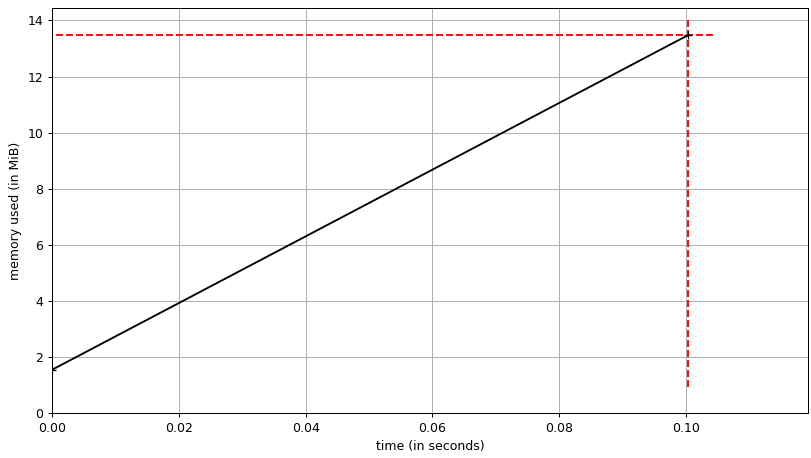
\includegraphics[width=\textwidth]{figures/experiments_figure_md5.png}
    \caption{Memory usage and runtime of the test script}
    \label{fig:memumd5}
\end{figure}
\subsection{Data capture}
The first process in our solution which could induce overheads is the data capture process and therefore, we want here to test its performances. In order to exclusively determine the memory usage and runtime of the data capture process, we activated the debug mode of the system to avoid the database writing process. 

The \autoref{fig:memuyoda} present the results of the memory profiler analysis. As it could be guessed, the process is inducing overheads. The execution time is now of 0.6s which represents a multiplication by 6 compared to the reference test. Concerning the memory the script now needs 27.6MiB of RAM which is more than the double of the original run.
\begin{figure}[h!]
  \centering
    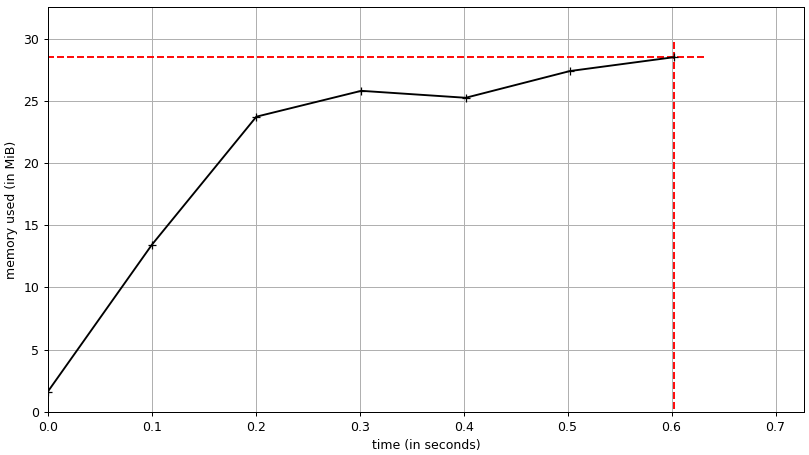
\includegraphics[width=\textwidth]{figures/experiments_figure_yoda.png}
    \caption{Memory usage and runtime with the Yoda system activated}
    \label{fig:memuyoda}
\end{figure}

These results could be seen as deceiving but in fact are inevitable because of the nature of our solution. Indeed, because we want to track the value of each variable at each line, the values are not overridden as in the normal run of the script. Instead, for each value, we store in the memory a copy of the variable and its data.

\subsection{Database writing}
The second process of interest which we want to test here is the database writing process. By activating this phase in the tool, we want to see if it is also inducing overheads. 

As it is shown in the \autoref{fig:memudb}, the introduction of the data writing process in our test is not inducing any significant additional memory usage which is now at the maximum around 29MiB. Nonetheless, the writing process induce a runtime overhead of 0.5s to now reach a total of 1.21s.
\begin{figure}[h!]
  \centering
    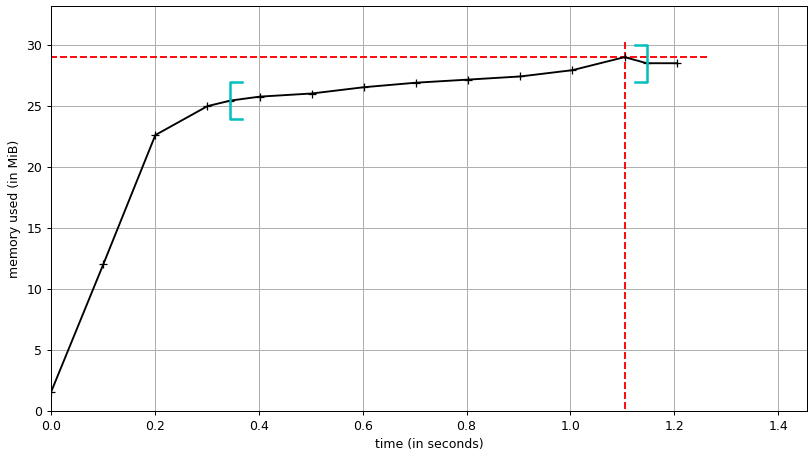
\includegraphics[width=\textwidth]{figures/experiments_figure_db.png}
    \caption{Memory usage and runtime with the database writing}
    \label{fig:memudb}
\end{figure}

\section{Concluding remarks}

In the \autoref{chap:relatedwork}, we already introduced some limitation of dynamic analysis tools, which is often heavy runtime overhead. We showed in the experiments that our solution is not an exception and induces even on a small script a heavier memory consumption and a significant runtime overhead. It has to be pointed out that the memory profiler is not an exact tool. In deed, according to \cite{Pedregos2016}, this module gets the memory consumption by querying the operating system kernel about the amount of memory the current process has allocated, which might be slightly different from the amount of memory that is actually used by the Python interpreter. Also, because of how the garbage collector works in Python the result might be different between platforms and even between runs.


\chapter{Conclusion} % Write in your own chapter title
\label{chap:conclusion}
\lhead{Chapter 5. \emph{Conclusion}} % Write in your own chapter title to set the page header

\section{Conclusion}
Lorem ipsum dolor sit amet, consectetur adipiscing elit, sed do eiusmod tempor incididunt ut labore et dolore magna aliqua. Ut enim ad minim veniam, quis nostrud exercitation ullamco laboris nisi ut aliquip ex ea commodo consequat. Duis aute irure dolor in reprehenderit in voluptate velit esse cillum dolore eu fugiat nulla pariatur. Excepteur sint occaecat cupidatat non proident, sunt in culpa qui officia deserunt mollit anim id est laborum.

\section{Future work}
String data --> complex data is not well handled
String data --> remove it from graph listing
Graphs --> zoom functionality
Long data is stored completely
Electron app ?

Lorem ipsum dolor sit amet, consectetur adipiscing elit, sed do eiusmod tempor incididunt ut labore et dolore magna aliqua. Ut enim ad minim veniam, quis nostrud exercitation ullamco laboris nisi ut aliquip ex ea commodo consequat. Duis aute irure dolor in reprehenderit in voluptate velit esse cillum dolore eu fugiat nulla pariatur. Excepteur sint occaecat cupidatat non proident, sunt in culpa qui officia deserunt mollit anim id est laborum.



%% ----------------------------------------------------------------
% Now begin the Appendices, including them as separate files


\appendix % Cue to tell LaTeX that the following 'chapters' are Appendices


%\input{./appendices/appendixA}	% Appendix Title

\printglossaries

\chapter{License of the software}
\label{appendix:license}

Copyright (c) 2016 DAVID CHENAUX

Permission is hereby granted, free of charge, to any person obtaining a copy of this software and associated documentation files (the "Software"), to deal in the Software without restriction, including without limitation the rights to use, copy, modify, merge, publish, distribute, sublicense, and/or sell copies of the Software, and to permit persons to whom the Software is furnished to do so, subject to the following conditions:

The above copyright notice and this permission notice shall be included in all copies or substantial portions of the Software.

THE SOFTWARE IS PROVIDED "AS IS", WITHOUT WARRANTY OF ANY KIND, EXPRESS OR IMPLIED, INCLUDING BUT NOT LIMITED TO THE WARRANTIES OF MERCHANTABILITY, FITNESS FOR A PARTICULAR PURPOSE AND NONINFRINGEMENT. IN NO EVENT SHALL THE AUTHORS OR COPYRIGHT HOLDERS BE LIABLE FOR ANY CLAIM, DAMAGES OR OTHER LIABILITY, WHETHER IN AN ACTION OF CONTRACT, TORT OR OTHERWISE, ARISING FROM, OUT OF OR IN CONNECTION WITH THE SOFTWARE OR THE USE OR OTHER DEALINGS IN THE SOFTWARE.


\clearpage

\addtocontents{toc}{\vspace{2em}}  % Add a gap in the Contents, for aesthetics
\backmatter

%% ----------------------------------------------------------------
\label{Bibliography}
\lhead{\emph{Bibliography}}  % Change the left side page header to "Bibliography"
\bibliographystyle{plainnat}  % Use the "unsrtnat" BibTeX style for formatting the Bibliography
\bibliography{thesis}  % The references (bibliography) information are stored in the file named "Bibliography.bib"
\clearpage
%% ----------------

\pagestyle{empty}
\label{Declaration}
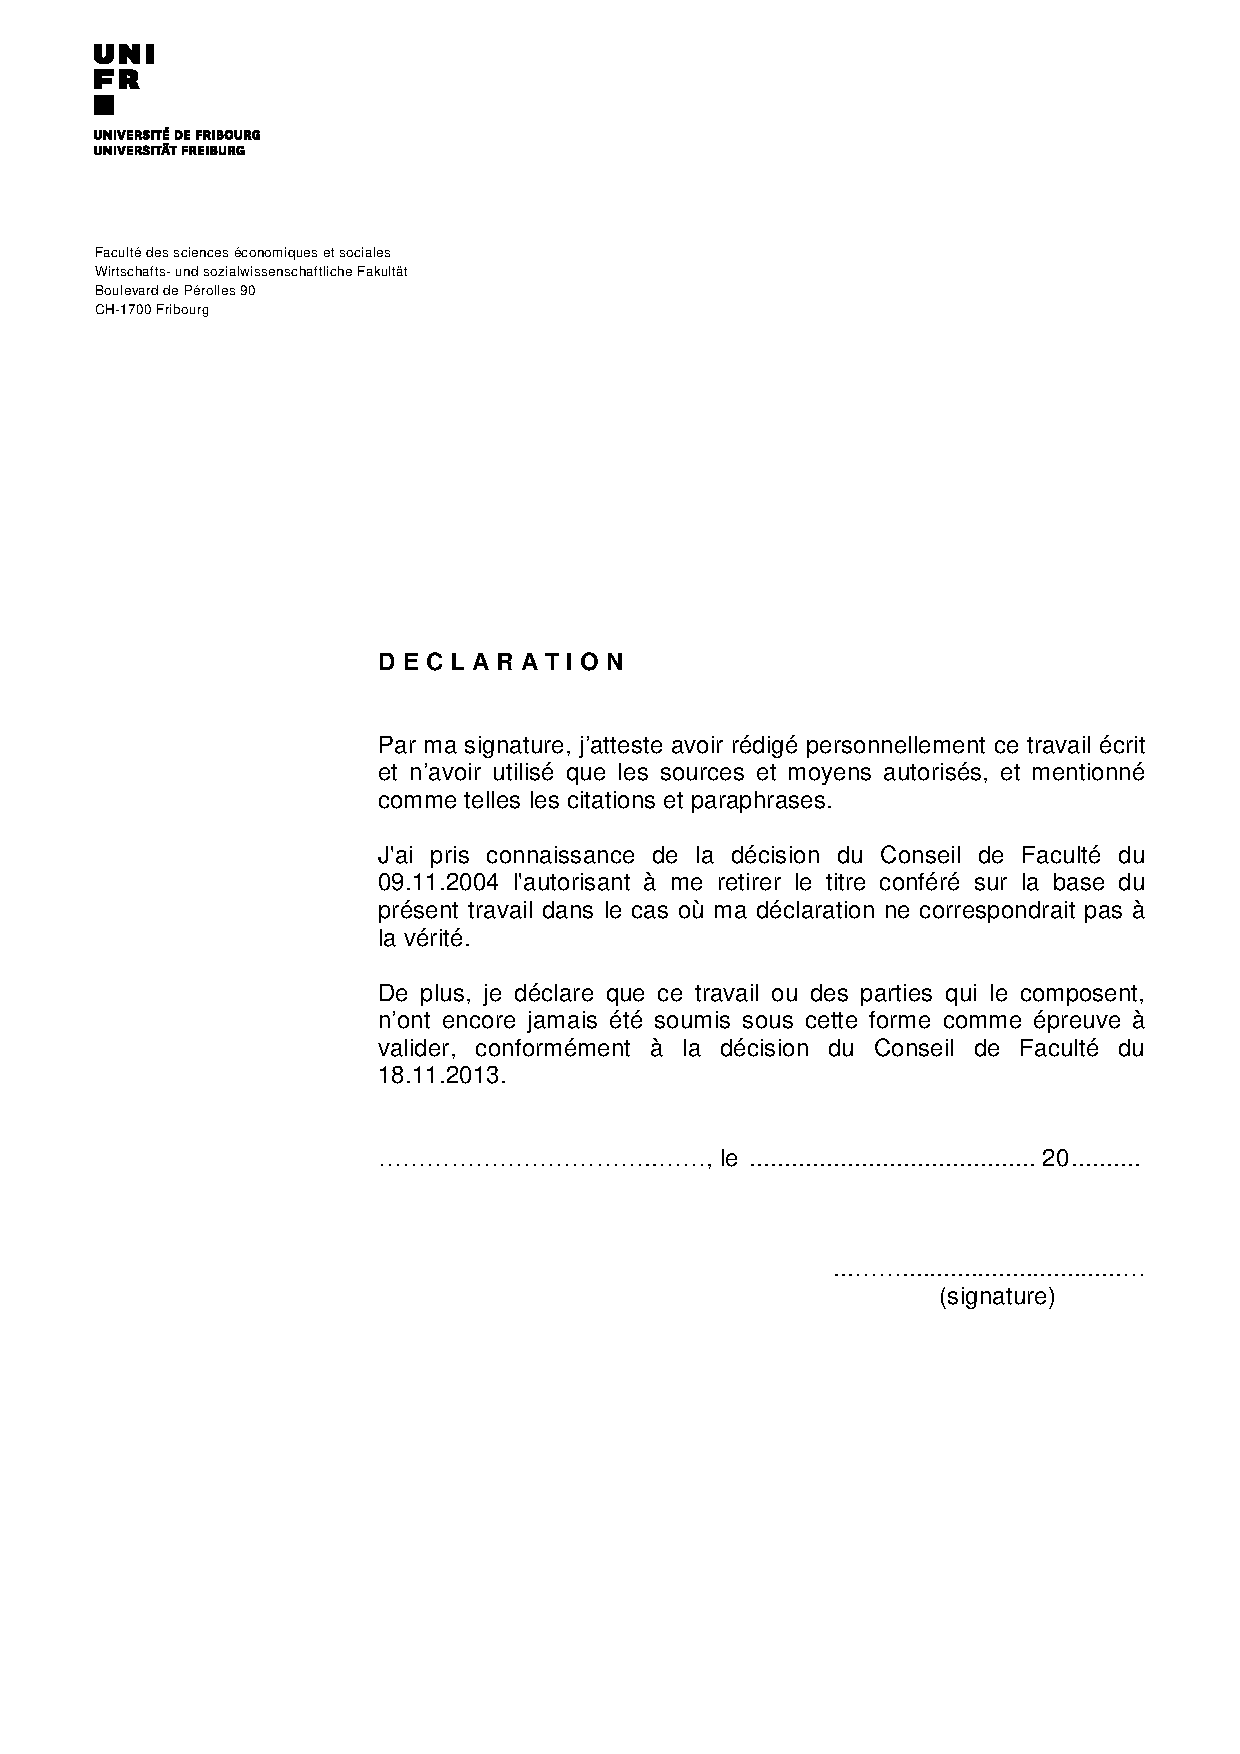
\includepdf[pages=-, offset=75 -75]{appendices/declaration.pdf}

\clearpage


%% ----------------------------------------------------------------
%\cleardoublepage
%\phantomsection
%\addcontentsline{toc}{chapter}{Index}
%\label{Index}
%\printindex


\end{document}  % The End
%% ----------------------------------------------------------------
